% ------------------------------------ ANALISI ----------------------------------

\chapter{Analisi}

\textsf{\small \textbf{Bullet Ballet} è un videogioco platform a scorrimento orizzontale, del genere \emph{Shoot 'em up} in 2D.}\\
\textsf{\small L'obiettivo del gioco è quello di realizzare più punti possibili per superare i propri record, in base alla distanza percorsa dal giocatore.}\\

\textsf{\small Ma non sarà tutto in discesa, il giocatore dovrà affrontare nemici con i più variegati equipaggiamenti, ostacoli di ogni sorta, varchi nella mappa e molto altro ancora...}\\
\textsf{\small Il giocatore potrà scegliere fra ben 4 mappe uniche e relative piattaforme in tema.}\\

\textsf{\small Inoltre, il giocatore potrà avvalersi a sua volta di effetti (bonus) sia positivi che negativi per poter sconfiggere le avversità che si presenteranno sul suo cammino.}\\

\textsf{\small Potrà, poi salvare tutte le sue statistiche di gioco.}\\

\section{Requisiti}

\textsf{\small L'applicazione mostra, all'avvio, un menù di gioco con le seguenti voci: \emph{New Game}, \emph{Settings}, \emph{Game Stats}, \emph{Quit}.}\\

\subsubsection{Requisiti funzionali}

\begin{itemize}
	\item \textsf{\small \emph{Mappa scorrevole}: Il giocatore potrà muoversi in una mappa a scorrimento orizzontale con uno sfondo statico.}
	\item \textsf{\small \emph{Menù di gioco}: Non appena lanciata l'applicazione, l'utente vedrà un menù di gioco con diverse opzioni tra cui potrà scegliere.}
	\item \textsf{\small \emph{Menù di pausa}: Il giocatore potrà mettere il gioco in pausa attraverso un dato pulsante della tastiera, scelto nelle impostazioni.}
	\item \textsf{\small \emph{Personaggio}: Il giocatore potrà scegliere un personaggio e muoverlo in partita.}
	\item \textsf{\small \emph{Nemici}: Verranno generati diversi nemici che il giocatore dovrà affrontare.}
	\item \textsf{\small \emph{Ostacoli e oggetti raccoglibili}: Verranno creati nella mappa degli ostacoli che bloccheranno la strada e degli oggetti che il giocatore potrà raccogliere per ricevere un (power up) bonus o un malus.}
	\item \textsf{\small \emph{Salvataggio del punteggio e classifica}: Terminata la partita, il punteggio di gioco potrà essere salvato e verrà generata una classifica finale.}
	\item \textsf{\small \emph{Suoni ed effetti sonori}: La durata della partita verrà accompagnata da una colonna sonora e agli effetti sonori prodotti dall'environment di gioco.}
	\item \textsf{\small \emph{Fisica di gioco}: Tutti le entità di gioco saranno dotate di una fisica ed una gravità propria.}
	\item \textsf{\small \emph{Criptazione dei files di gioco}: Tutti i files di gioco: livelli, statistiche e impostazioni verranno criptate per evitare che il giocatore possa modificarle.}
\end{itemize}

\subsection{Requisiti non funzionali e opzionali}

\textsf{\small Questi requisiti non concorrono a far parte delle funzionalità minime del gioco e per questioni di tempistica e/o di budget non verranno necessariamente implementate.}\\

\begin{itemize}
	\item \textsf{\small \emph{Oggetti dinamici}: ovvero oggetti che si muovono e che hanno una animazione.}
	\item \textsf{\small \emph{Market}: per poter comprare/vendere skin (mimetiche) di gioco con valuta reale o in gioco. (o fittizia del gioco)}
	\item \textsf{\small \emph{Modalità storia}: una modalità con una storia di gioco e diversi livelli che il giocatore dovrà sbloccare per poter continuare ad avanzare nel gioco.}
	\item \textsf{\small \emph{Statistiche di gioco}: Varie statistiche di gioco, mostrate in diversi diagrammi.}
	\item \textsf{\small \emph{Difficoltà di gioco}: Possibilità di scegliere diverse difficoltà che potrebbero aggiungere numero di nemici/ostacoli/oggetti di varia natura e/o incrementare la loro vita.}
\end{itemize}

\section{Analisi e modello del dominio}

\textsf{\small L'applicazione fornisce un giocatore che tramite input dell'utente può essere spostato a destra, a sinistra e farlo saltare. Il quale, potrà interagire con le varie entità, sia statiche che dinamiche del gioco, quali \emph{nemici}, \emph{armi}, \emph{monete}, \emph{items}, \emph{ostacoli}.
Ognuna di queste entità interagirà in maniere differenti col player: }\\

\begin{itemize}
	\item \textsf{\small \emph{Enemy}, ostacolerà il player a colpi di mitra.} %TODO: da modificare.
	\item \textsf{\small \emph{Item}, una volta raccolta dal player, gli fornirà o un \textbf{bonus}, come una vita extra oppure un \textbf{malus} come un effetto di veleno per tot tempo.}
	\item \textsf{\small \emph{monete}, faranno aumentare il punteggio e il numero di monete del gioco da usare nel mercato per poter comprare nuove skins, in game-items, ecc...}
	\item \textsf{\small \emph{Armi}, dopo essere state raccolte verranno equipaggiate al giocatore.}
	\item \textsf{\small \emph{Ostacoli}, se il player ci si scontrerà, subirà del danno.}
\end{itemize}

\textsf{\small Il gioco si conclude quando e se il player riesce a raggiungere la fine della mappa senza morire.}
\textsf{\small Se il player viene ucciso prima di raggiungere la fine, allora viene eliminato e la partita è persa.}\\

\textsf{\small Ogni round è a sé stante, finita la partita, al player verrà assegnato un punteggio e potrà scegliere se rigiocare od uscire.}\\

%TODO: aggiungere UML.

%\begin{landscape}
	\begin{figure}[h]
		\centering{}
		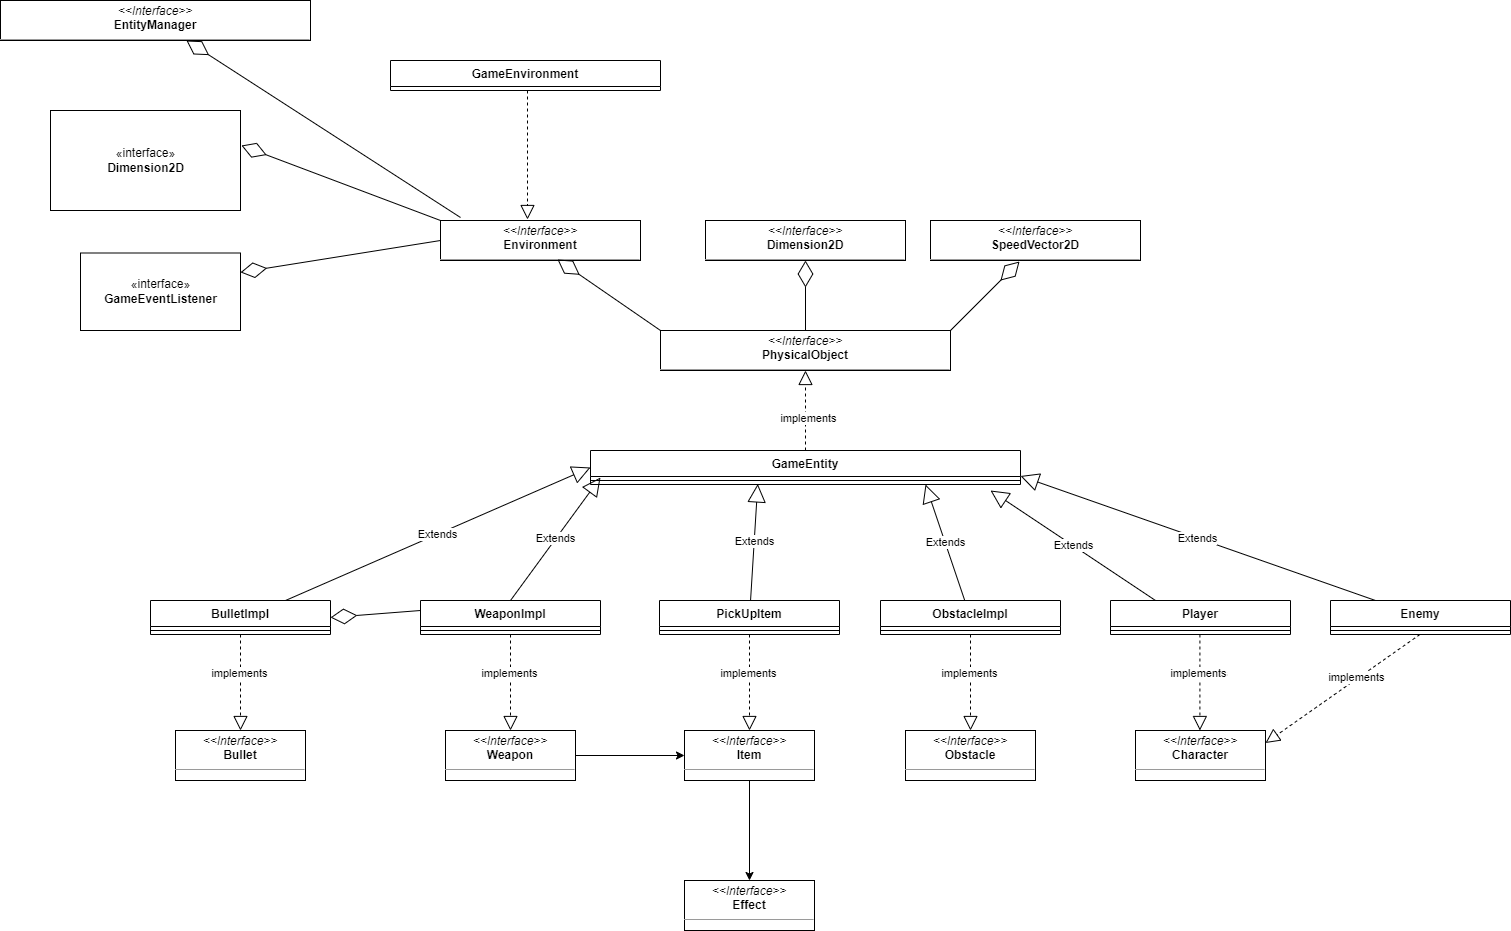
\includegraphics[width=1.2\linewidth]{./img/model.png}
		\caption{Schema UML dell'analisi del problema, con rappresentate le entità principali ed i rapporti fra loro.}
		\label{img:analysis}
	\end{figure}
%\end{landscape}
